
\chapter{Modules}

\begin{itemize}
\item Functions allow us to parcel up pieces of code so that they can be reused throughout a program.
\item Modules provides a means of collecting sets of functions together so that they can be used by any number of programs.
\item Packages group sets of modules because their moduels provide related functionality or because they depend on each other.
\end{itemize}


\begin{tcolorbox}
  It is important to be aware of what the library has to offer, since using predefined functionality makes programming much faster than creating everything from scratch.
\end{tcolorbox}


\section{Modules and packages}

Several syntaxes can be used when importint:
\begin{tcolorbox}
\begin{verbatim}
import importable
import importable1, importable2, ..., importableN
import importable as preferred_name

from importable import object as preferred_name
from importable import object1, object2, ..., objectN
from importable import *
\end{verbatim}
\end{tcolorbox}


In the last syntex, the * means ``import everything that is not private'',
which in practical terms means
either every object in the module is imported except for those whose names begin with a leading underscore, or,
if the module has a global \verb|__all__| variable that holds a list of names, that all the objects named in the \verb|__all__| variable are imported.






\begin{tcolorbox}
  How does Python know where to look for the modules and packages that are imported?

  The built-in \verb|sys| module has a list called \verb|sys.path| that holds a list of the directories that consistutes the \keyword{Python path}.
  The first directory is the directory that contains the program itself, even if the program was invoked from another directory.
  If the PYTHONPATH environment variable is set, the paths specified in it are the next ones in the list.
  The final paths are those needed to access Python’s standard library --- these are set when Python is installed.

  When we first import a module, if it isn’t built-in, Python looks for the module in each path listed in \verb|sys.path| in turn. 
\end{tcolorbox}


\begin{figure}[!ht]
  \centering
  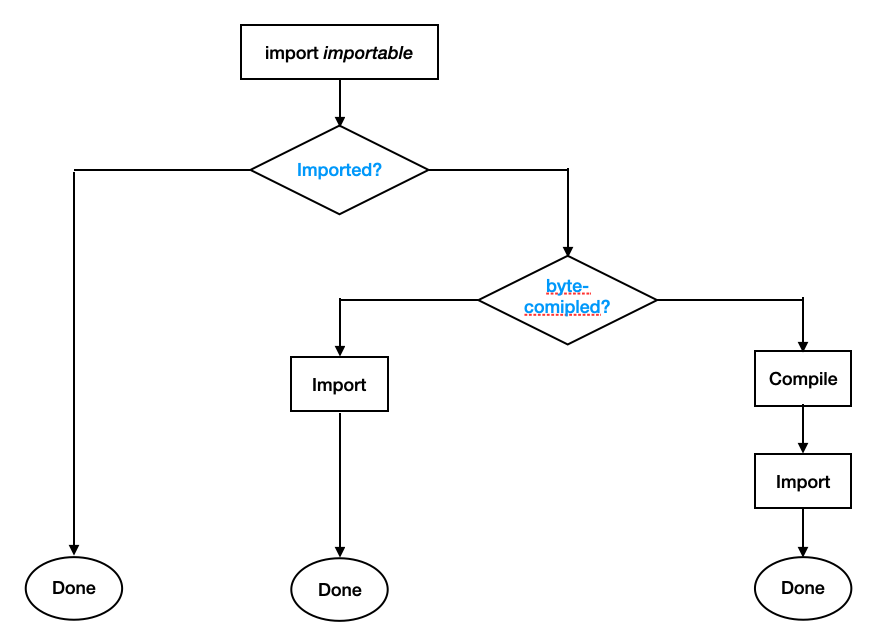
\includegraphics[width=\textwidth]{pics/import}
  \caption{Import}
\end{figure}


Using byte-code compiled files leads to faster start-up times since the interpreter only has to load and run the code, rather than load, compile, (save if possible),and run the code;runtimes are not affected, though.
WhenPythonis installed, the standard library modules are usually byte-code compiled as part of the installation process.


\subsection{Packages}

A package is simply a directory that contains a set of modules and a file called \verb|__init__.py|.



In some situations it is convenient to load in all of a \keyword{package}’s modules using a single statement.
To do this we must edit the \keyword{package}’s \verb|__init__.py| file to contain a statement which specifies which modules we want loaded.
This statement must assign a list of module names to the special variable \verb|__all__|.



This syntax can also be applied to a module in which case all the functions, variables, and other object defined in the module (appart from those whose names begin with a leading underscore) will be imported.
If we want to control exactly what is imported, we can define an \verb|__all__| list in the module itself.




\subsection{Custom modules}

\subsubsection{The TextUtil module}



\keyword{TextUtil.py}:

\begin{lstlisting}
#!/usr/bin/env python3
# Copyright
"""
This module provides a few string manipulation functions.

>>> is_balanced("(Python (is (not (lisp))))")
True
>>> shorten("The Crossing", 10)
'The Cro...'
>>> simplify(" some  text   with spurious   whitespace   ")
'some text with spurious whitespace'
"""

import string


def simplify(text, whitespace=string.whitespace, delete=''):
    r"""Returns the text with multiple spaces reduced to single spaces

    The whitespace parameter is a string of characters, each of which
    is considered to be a space.
    If delete is note empty it should be a string, in which case any
    characters in the delete string are excluded from the resultant
    string.

    >>> simplify(" this    and\n that\t too")
    'this and that too'
    >>> simplify("  Washington    D.C.\n")
    'Washington D.C.'
    >>> simplify("  Washington   D.C.\n", delete=',;:.')
    'Washington DC'
    >>> simplify(" disemvoweled ", delete="aeiou")
    'dsmvwld'
    """
    result = []
    word = ""
    for char in text:
        if char in delete:
            continue
        elif char in whitespace:
            if word:
                result.append(word)
                word = ""
        else:
            word += char
    if word:
        result.append(word)
        return " ".join(result)


def is_balanced(text, brackets="()[]{}<>"):
    """Returns True if all the brackets in the text are balanced

    For each pair of brackets, the left and right bracket characters
    must be different.

    >>> is_balanced("no brackets at all")
    True
    >>> is_balanced("<b>bold</b>")
    True
    >>> is_balanced("[<b>(some {thing}) goes</b>]")
    True
    >>> is_balanced("<b>[not (where {it}) is}]</b>")
    False
    >>> is_balanced("(not (<tag>(like) (anything)</tag>)")
    False
    """
    counts = {}
    left_for_right = {}
    for left, right in zip(brackets[::2], brackets[1::2]):
        assert left != right, "the bracket characters must differ"
        counts[left] = 0
        left_for_right[right] = left
    for c in text:
        if c in counts:
            counts[c] += 1
        elif c in left_for_right:
            left = left_for_right[c]
            if counts[left] == 0:
                return False
            counts[left] -= 1
    return not any(counts.values())


def shorten(text, length=25, indicator="..."):
    """Returns text or a truncated copy with the indicator added

    text is any string; length is the maximum length of the returned
    string (including any indicator); indicator is the string added at
    the end to indicate that the text has been shortened

    >>> shorten("Second Variety")
    'Second Variety'
    >>> shorten("Voices from the Street", 17)
    'Voices from th...'
    >>> shorten("Radio Free Albemuth", 10, "*")
    'Radio Fre*'
    """
    if len(text) > length:
        text = text[:length - len(indicator)] + indicator
    return text


if __name__ == '__main__':
    import doctest

    doctest.testmod()
  
\end{lstlisting}


To use the our module:
\begin{lstlisting}
import TextUtil
text = " a puzzling conundrum "
text = TextUtil.simplify(text) # text == 'a puzzling conundrum'
\end{lstlisting}


If we want our module to be available to a particular program, we just need to put our module in the same directory as the program.
If we want our module to be available to all our programs, there are several approaches:
\begin{enumerate}
\item put the module in the Python distribution's \verb|site-packages| subdirectory
\item create a directory specifically for the custom modules, and set the \verb|PYTHONPATH| environment variable to this directory
\item put the module in the local site-packages subdirectory (~/.local/lib/python3.1/site-packages)
\end{enumerate}

The second and third approaches have the advantage of keeping our own code separate from the official installation.



Doctesting is done by:
\begin{lstlisting}
if __name__ == '__main__':
    import doctest

    doctest.testmod()
\end{lstlisting}

Whenever a module is imported Python creates a variable for the module called \verb|__name__| and stores the module’s name in this variable.
A module’s name is simply the name of its \verb|.py| file but without the extension.
So in this example, when the module is imported \verb|__name__| will have the value "TextUtil", and the if condition will not be met, so the last two lines will not be executed.
This means that these last three lines have virtually no cost when the module is imported.



Whenever a \verb|.py| file is run Python creates a variable for the program called \verb|__name__| and sets it to the string "\verb|__main__|".
So if we were to run \verb|TextUtil.py| as though it were a program, Python will set \verb|__name__| to "\verb|__main__|" and the if condition will evaluate to True and the last two lines will be executed.




\section{Overview of Python’s standard library}

The standard library is the library installed when you install Python.
You do not need to install the library separately.
Python's standard library is generally described as ``batteries included''.
The third-party library is the library you should install by yourself.

\subsection{Strings}

\begin{lstlisting}
import sys
import io

print('hello', file=sys.stdout)
print('hello', file=sys.stderr)
sys.stdout.write('world')

fh = open('text.txt', 'w')
print('hello world', file=fh)

string_io = io.StringIO()
sys.stdout = string_io

for i in range(100):
    print('hello' + i)

sys.stdout = sys.__stdout__  # recover the default sys.stdout
print(string_io.getvalue())  # get the value in string io
\end{lstlisting}

\subsection{Dates and Times}

\begin{lstlisting}
import datetime
import time

# current seconds
current_second = time.time()

# current date and time
current_time = datetime.datetime.now()

# current struct time
current_struct_time = time.localtime()

# format from struct time
string_time = time.strftime('%Y-%m-%d %H:%M:%S', current_struct_time)

# struct time from string
struct_time = time.strptime('2021-02-04 11:07:09', '%Y-%m-%d %H:%M:%S')

# seconds from struct time
seconds = time.mktime(current_struct_time)  
\end{lstlisting}

\subsection{Algorithms and collection data types}

\begin{lstlisting}
import heapq

heap = []
heapq.heappush(heap, (5, 'a'))
heapq.heappush(heap, (2, 'b'))
heapq.heappush(heap, (4, 'c'))

for _ in range(len(heap)):
    print(heapq.heappop(heap))

h = [1, 5, 11, 10, 3, 6, 20, 8, 7, 2, 9]
heapq.heapify(h)
for _ in range(len(h)):
    print(heapq.heappop(h))  
\end{lstlisting}


\subsection{File formats, encodings, and data persistence}

\begin{lstlisting}
import base64

binary = open('ali.png', 'rb').read()
ascii_text = ''
for i, c in enumerate(base64.b64encode(binary)):
    if i and i % 68 == 0:
        ascii_text += '\\\n'
    ascii_text += chr(c)
print(ascii_text)

binary = base64.b64decode(ascii_text)
open('ali_copy.png', 'wb').write(binary)
\end{lstlisting}


\begin{lstlisting}
import tarfile
import string
import sys
import os

BZ2_AVAILABLE = True
try:
    import bz2
except ImportError:
    BZ2_AVAILABLE = False

# absolute path is not permitted
UNTRUSTED_PREFIXES = tuple(['/', '\\'] + [c + ':' for c in string.ascii_letters])


def untar(archive):
    tar = None
    try:
        tar = tarfile.open(archive)
        for member in tar.getmembers():
            if member.name.startswith(UNTRUSTED_PREFIXES):
                print('untrusted prefix, ignoring', member.name)
            elif '..' in member.name:
                print('suspect path, ignoring', member.name)
            else:
                tar.extract(member)
                print('unpacked', member.name)
    except (tarfile.TarError, EnvironmentError) as err:
        print(err)
    finally:
        if tar is not None:
            tar.close()


def error(message, exit_status=1):
    print(message)
    sys.exit(exit_status)  
\end{lstlisting}


